\documentclass[buriama8_dp.tex]{subfiles}
\begin{document}

\chapter{Experiments}

All steps in implementation of the solution were verified by experiments. We conducted both simulated experiments and experiments on a real robotic arm.

\section{Benchmark environment}
\label{sec:exp_cpp_env}

We created a benchmark environment representing an obstacle in front of the robot. The environment is represented in a grid \(10 \times 10 \times 5\) cells. We also tested the algorithms in free space, to evaluate if they produce paths reasonable to a human eye.

The environment contains two obstacles, a floor-standing object and an overhang above the object, with enough space for the robot to pass through. A single plane extracted from the full 3D environment is used as the 2D benchmark for the coverage algorithm. The planar environment is illustrated in Figure~\ref{fig:2d_env}.

\begin{figure}[htp]
  \centering
  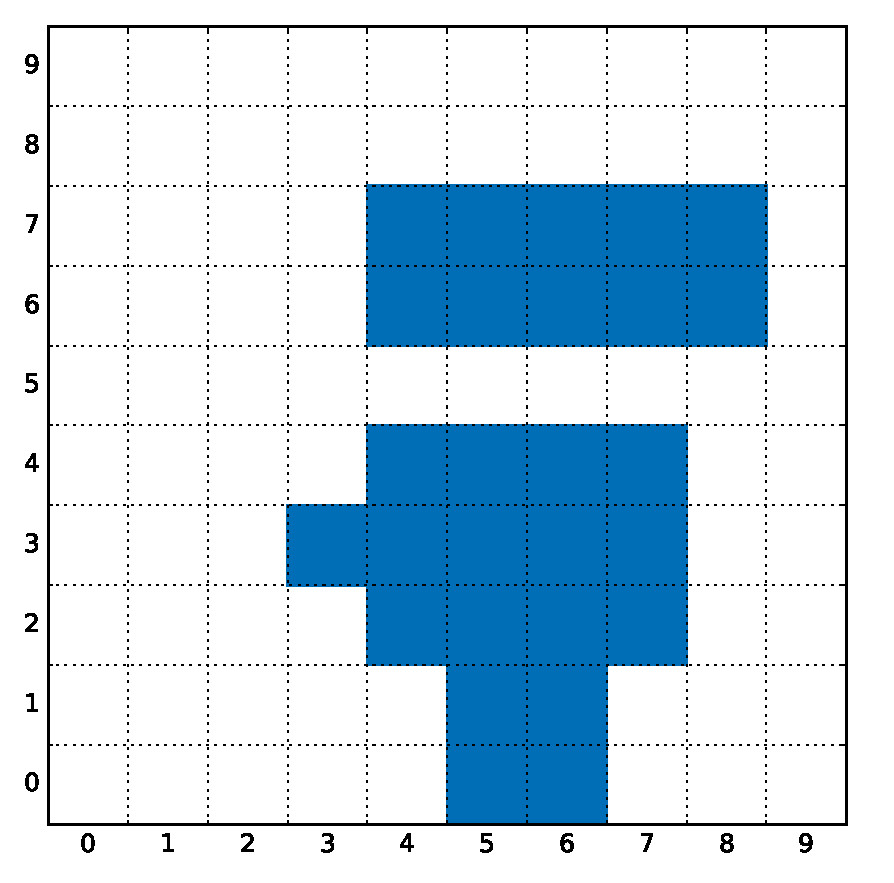
\includegraphics[width=7cm]{2d_coverage_env.pdf}
  \caption[2D benchmark environment]{The 2D benchmark environment for CPP algorithms. The environment is depicted as a vertical slice as seen by the robot; the \uvz{floor} is at the bottom}
  \label{fig:2d_env}
\end{figure}

In simulating coverage algorithms, we ignore the arm collision checking with previously discovered obstales. This is accounted for when we simulate the whole arm.

\section{Simulated coverage algorithms}
\label{sec:exp_sim_coverage}

To test the performance of CPP algorithms we implemented, we peformed experiments to determine how well the methods perform in unknown environments in both 2 and 3 dimensions. Each of the algorithms was run in \REV{an} empty 2D environment to test it in the simplest setting, followed by a run in the benchmark environment described in Section~\ref{sec:exp_cpp_env} Because of the generalization scheme used to adapt the algorithm to explore 3D space, 2D environment is represented in 3D as a grid with only one depth layer.

\subsection{Two dimensions}
\label{subsec:2d_sim}

Running the compact space heuristic algorithm in the 2D environment, we obtained paths depicted in Figure~\ref{fig:heur_2d_coverage}.

\begin{figure}[ht]
  \centering
  \begin{subfigure}[t]{0.49\textwidth}
    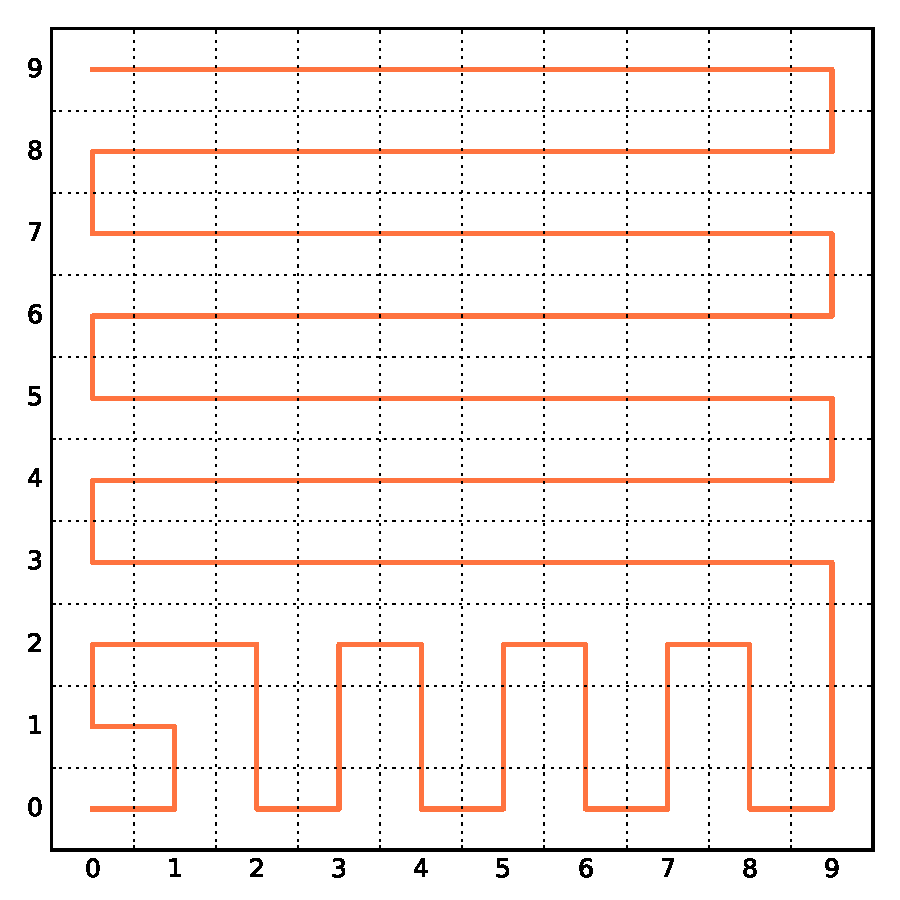
\includegraphics[width=\textwidth]{2d_coverage_heur_empty.pdf}
    \caption{}
    \label{fig:heur_2d_empty}
  \end{subfigure}
  \begin{subfigure}[t]{0.49\textwidth}
    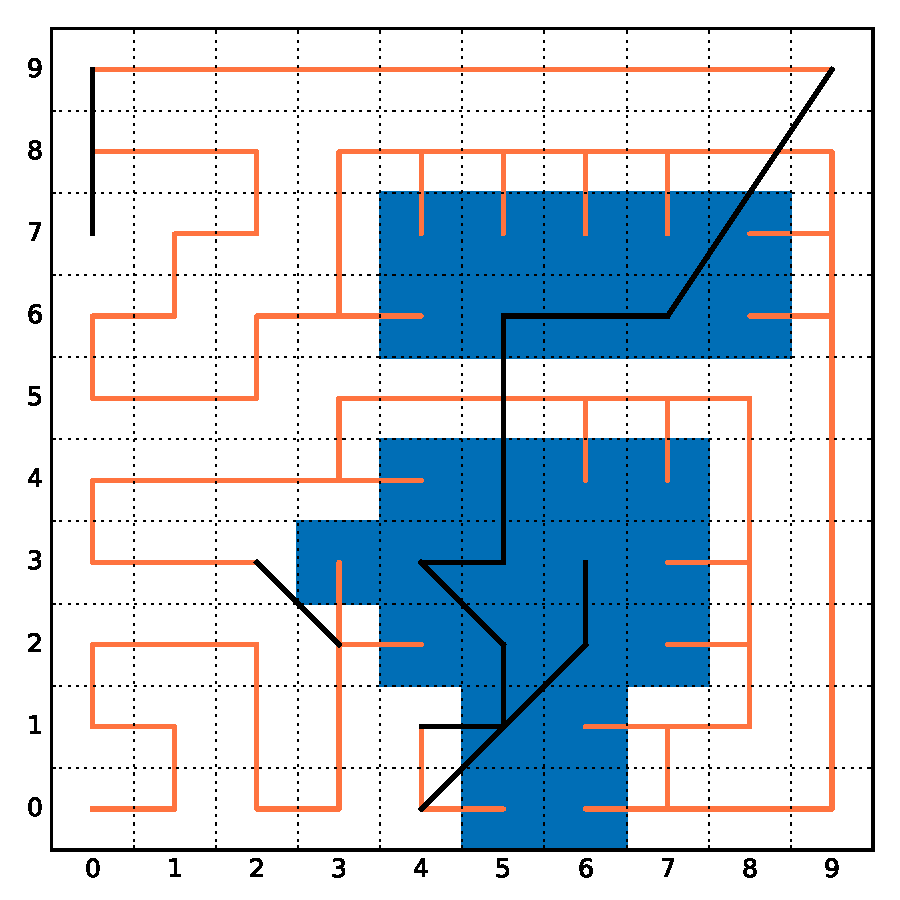
\includegraphics[width=\textwidth]{2d_coverage_heur.pdf}
    \caption{}
    \label{fig:heur_2d_env}
  \end{subfigure}
  
  \caption[Coverage path -- compact space heuristic in 2D]{Coverage path generated by them compact space heuristic in an empty (a) and in the benchmark environment (b). The path starts at \([0,0]\) and is depicted in orange, with transitions to nearest unexplored field depicted in black. The path plot is perturbed by a small amount to let the reader follow it more easily}
  \label{fig:heur_2d_coverage}
\end{figure}

The results in empty space are reasonable. The generated path closely resembles the boustrophedon pattern used in human-designed algorithms. The already explored space is kept compact, as was the aim of the heuristic. The length of the generated path is 9.9\,m, which is the optimal value since no cell was explored twice. This is allowed by the even size of the environment; in case of odd environment width, the lower zig-zag terminates in the lower-right corner and the robot then has to return back to the yet unexplored portion of the environment, travelling through the already known fields again.

In the benchmark environment, we can see that the path starts the same as in the empty environment. When the obstacle is encountered, we can indentify the algorithm following the other incentive it has -- exploring space near known obstacles. This leads to obstacle-circling, after which the obstacle limits are quickly determined. The length of the path is 1.25\,m. \TODO{elaborate}

\subsection{Three dimensions}
\label{subsec:3d_sim}

The results of running the coverage algorithm are shown in Figure~\ref{fig:heur_3d_coverage}.

\begin{figure}[ht]
  \centering
  \begin{subfigure}[t]{0.48\textwidth}
    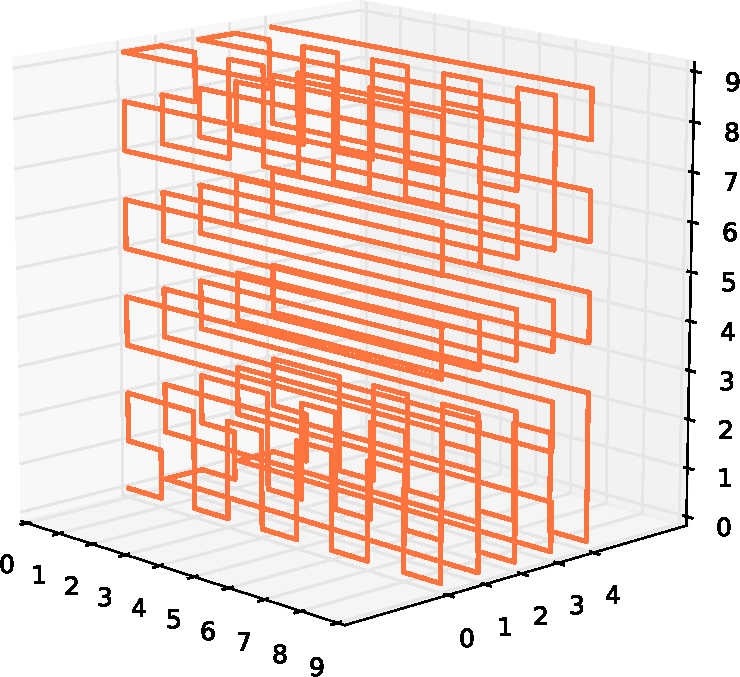
\includegraphics[width=\textwidth]{3d_coverage_heur_empty-cropped.pdf}
    \caption{}
    \label{fig:heur_3d_empty}
  \end{subfigure}
  \;
  \begin{subfigure}[t]{0.48\textwidth}
    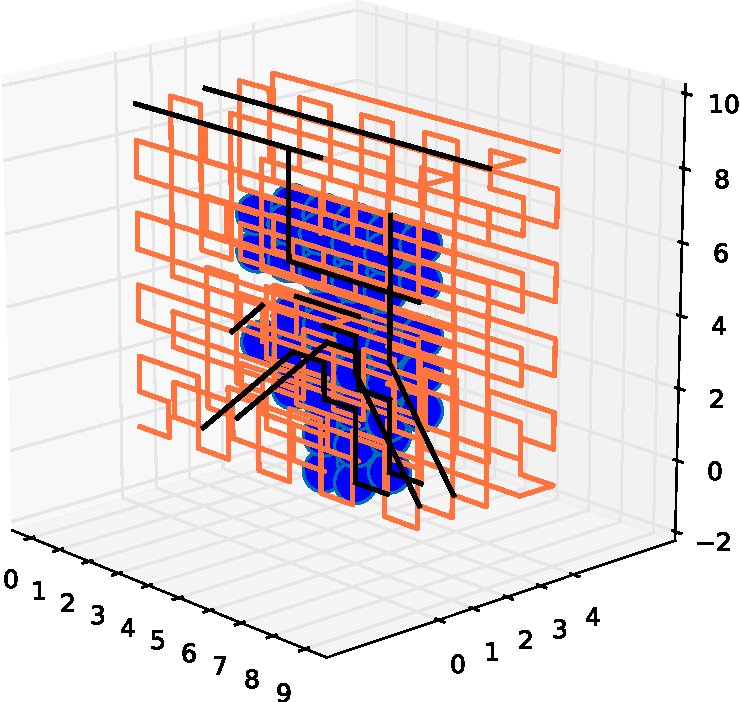
\includegraphics[width=\textwidth]{3d_coverage_heur-cropped.pdf}
    \caption{}
    \label{fig:heur_3d_env}
  \end{subfigure}
  
  \caption[Coverage path -- compact space heuristic in 3D]{}
  \label{fig:heur_3d_coverage}
\end{figure}

Expectedly, the algorithm runs in 3D space as well as in two dimensions. In both cases, we can observe the layers in which the environment has been explored. In the empty environment, the algorithm starts and ends on opposite sides, and thus the layers are identical, only mirrored. The found path is again optimal with length of 49.9\,m.

When obstacles are present, the coverage path is different in each layer partly because of the varying obstacles, partly because of different entry points, as one layer starts precisely where the other has ended. The path is 56.3\,m long.


\section{Simulated arm experiments}
\label{sec:exp_sim_arm}

\section{Real arm experiments}
\label{sec:exp_real_arm}



\end{document}


%%% Local Variables:
%%% mode: latex
%%% TeX-master: "buriama8_dp"
%%% End:
